% Use the following line  only  if you're still using LaTeX 2.09.
%\documentstyle[icml2014,epsf,natbib]{article}
% If you rely on Latex2e packages, like most moden people use this:
\documentclass{article}
% use Times
\usepackage{times}
 % For figures
\usepackage{graphicx} % more modern
%\usepackage{epsfig} % less modern
\usepackage{subfigure} 
\usepackage{footnote}
\usepackage{amsfonts}
\usepackage{mdframed}

% For citations
\usepackage{natbib}
\usepackage{comment}
\usepackage{multirow}

\usepackage{float}

\floatstyle{plain} % optionally change the style of the new float
\newfloat{code}{H}{myc}

% For algorithms
\usepackage{algorithm}
\usepackage{algorithmic}
\usepackage{amsmath}
\usepackage{listings}

\lstset{language=Python,
  basicstyle=\ttfamily\footnotesize,
  keywordstyle=\color{blue}\ttfamily,
  stringstyle=\color{red}\ttfamily,
  commentstyle=\color{green}\ttfamily,
  aboveskip=0pt,
  belowskip=0pt,
  breaklines=true
}

\setlength{\abovedisplayskip}{0cm}
\setlength{\belowdisplayskip}{0cm}

\usepackage{mathtools}


\newcommand\myeq{\stackrel{\mathclap{\normalfont\mbox{{\tiny def}}}}{=}}


\usepackage[compact]{titlesec}
\titlespacing{\section}{0pt}{0.5ex}{0.3ex}
\titlespacing{\subsection}{0pt}{0.2ex}{0ex}
\titlespacing{\subsubsection}{0pt}{0.1ex}{0ex}

\newcommand{\startcompact}[1]{\par\vspace{-0.75em}\begin{#1}%
  \allowdisplaybreaks\ignorespaces}

\newcommand{\stopcompact}[1]{\end{#1}\ignorespaces}

\usepackage{paralist}

\makeatletter
\ifcase \@ptsize \relax% 10pt
  \newcommand{\miniscule}{\@setfontsize\miniscule{4}{5}}% \tiny: 5/6
\or% 11pt
  \newcommand{\miniscule}{\@setfontsize\miniscule{5}{6}}% \tiny: 6/7
\or% 12pt
  \newcommand{\miniscule}{\@setfontsize\miniscule{5}{6}}% \tiny: 6/7
\fi
\makeatother

\newcommand {\aplt} {\ {\raise-.5ex\hbox{$\buildrel<\over\sim$}}\ }

\newcommand{\eqn}[1]{Eqn.~\ref{eqn:#1}}
\newcommand{\fig}[1]{Fig.~\ref{fig:#1}}
\newcommand{\tab}[1]{Table~\ref{tab:#1}}
\newcommand{\secc}[1]{Section~\ref{sec:#1}}
\def\etal{{\textit{et~al.~}}}
\newcommand{\BigO}[1]{\ensuremath{\operatorname{O}\left(#1\right)}}
\usepackage[symbol*]{footmisc}

\DefineFNsymbolsTM{myfnsymbols}{% def. from footmisc.sty "bringhurst" symbols
  \textasteriskcentered *
  \textdagger    \dagger
  \textdaggerdbl \ddagger
  \textsection   \mathsection
  \textbardbl    \|%
  \textparagraph \mathparagraph
}%


% As of 2011, we use the hyperref package to produce hyperlinks in the
% resulting PDF.  If this breaks your system, please commend out the
% following usepackage line and replace \usepackage{icml2014} with
% \usepackage[nohyperref]{icml2014} above.
\usepackage{hyperref}

% Packages hyperref and algorithmic misbehave sometimes.  We can fix
% this with the following command.
\newcommand{\theHalgorithm}{\arabic{algorithm}}

% Employ the following version of the ``usepackage'' statement for
% submitting the draft version of the paper for review.  This will set
% the note in the first column to ``Under review.  Do not distribute.''
%\usepackage{icml2014} 
% Employ this version of the ``usepackage'' statement after the paper has
% been accepted, when creating the final version.  This will set the
% note in the first column to ``Proceedings of the...''
\usepackage[accepted]{icml2014}



\begin{document} 

\twocolumn[
\icmltitle{Learning to Reason\\{\small PhD Thesis Proposal}}

\icmlauthor{Wojciech Zaremba}{woj.zaremba@gmail.com}
\vskip +0.1in
\icmlauthor{Advisors:}{}
\vskip +0.03in
\icmlauthor{Rob Fergus}{fergus@cs.nyu.edu}
\vskip +0.03in
\icmlauthor{Yann LeCun}{yann@cs.nyu.edu}
\icmladdress{New York University}

\icmlkeywords{computer vision, convolutional neural networks, recurssive neural networks, natual language processing, recurrent neural networks, language model, LSTMs, program understanding, artificial intelligence}

\vskip 0.3in
]

\begin{abstract}

Neural networks proven to be a very powerful models for object recognition \cite{krizhevsky2012imagenet}, 
natural language processing \cite{mikolov2012statistical}, speech recognition \cite{graves2013speech}, and many others \cite{sutskever2014sequence}. 
However, there is still a huge gap between them, and an intelligent systems. 
I identify several potential unaddressed skills, which intelligent systems should possess: 
(1) reasoning abilities, (2) capability to integrate with external interfaces and (3) small sample complexity. My research focuses on tackling this problems. 

\end{abstract} 

\section{Introduction}
It's clear that by improving performance of current statistical learning systems, 
we won't be able to make them intelligent. Even if our object recognition system would yield
$0\%$ of prediction error, they wouldn't be intelligent. Same applies to speech 
recognition systems, machine translation and others. This work asks what skills are necessary for statistical
learning system to become ``intelligent''. Moreover, it attempts to address this remaining unaddressed skills. 


I believe, that crucial, poorly addressed skills that intelligent system has to poses are
(1) reasoning abilities, (2) capability to integrate with external interfaces and (3) small sample complexity. 
I would like to address all this problems within a seamless system. The same system should be used across
different tasks to verify its empirical universality.


I have partially addressed some of proposed problems. I will make clear over the further part of this proposal, 
which parts have been addressed, and which are future goals.



\section{Reasoning abilities}

\textit{Reasoning} - ``the process of forming conclusions, judgments, or inferences from facts or 
premises''\footnote{Definition from \url{http://dictionary.reference.com/browse/reasoning}}.
\\
\\
System that can reason should be able to understand high level concepts like 
\begin{itemize}
 \item scope
 \item being able to instantly memorize 
 \item conditioning
 \item nesting
 \item repetitions
 \item and many more
\end{itemize}
Each of this skills could be solved in particular domain. However, solving problem in a single domain
limits use of such system,
and assumes that we know a priori all possible scenarios. 
Moreover, I think that, intelligent reasoning system cannot be based only on predefined rules. 
Intelligent system has to be based on pattern matching, and application of learnt heuristic algorithms. 


There are many domains where we can test if our system can reason, and if it's able to learn postulated concepts. Eventually,
I would like to use the same tools for all domains. 
Domains of my interest are learning about computer programs, and 
proving mathematical theorems.
This domains are rich in scoping, branching, nesting, pattern repetition, and so on. Drawing
high level conclusions in such domains requires sophisticated reasoning skills.

\subsection{Reasoning in computer programs}
The first reasoning task that I am interest in is to train statistical models meaning of computer programs.
I propose one instance of program understanding.
Task is to take a program as an input (in our case character-by-character), and predict program evaluation. 
Prediction of program evaluation requires understanding every single operand of a program. For instance, in case of
addition it 
involves bit shifts, and memorization of operations on digits. Moreover, programs contain variable assignment, if-statements, and so on.
We were able partially to address postulated problem
\cite{zaremba2014execute}.
Figure \ref{fig:prog} shows
an exemplary program, target for such program, and prediction that we obtained with recurrent neural network.

\begin{figure}
  \begin{code}
  \begin{mdframed}
  {\bf Input:}
  \begin{lstlisting}
  f=(8794 if 8887<9713 else (3*8334))
  print((f+574))
  \end{lstlisting} 
  {\bf Target:} 9368. \\
  {\bf Model prediction:} 9368. 
  \end{mdframed}
  \end{code}
  \caption{An exemplary program that we take as an input. Task is to predict program evaluation. We have 
  achieved high performance on this task \cite{zaremba2014execute}.}
  \label{fig:prog}
\end{figure}


Current results are promising, however they are very limited. We are able to deal with programs
that can be evaluated by reading them once from left-to-right. Generic programs are not like that.
Our reasoning system has to be able to evaluate for arbitrary long time, if
task requires it. Moreover, it shouldn't be limited by finite memory size. Memory should be available
as an interface (Section \ref{sec:interface}).


\subsection{Reasoning in mathematics}
It's known that theorem proving is an intractable task in computational sense. 
However, humans are able to prove theorems. They have to employ a-prior
knowledge. They fit known mathematical ``tricks'' to the new problem.


More formally, we can think about proofs as a multiple axioms application that starts with
hypothesis that we want to prove. This way mathematical skills can be perceived as 
learning prior over trees of axioms. This prior ``suggests'' us which sequence of axioms is more
likely to lead to the theorem proof. 


My interest lies in training statistical machine learning system to learn such priors. 
We have started with very constrained mathematical domain. 
We learn here prior over mathematical identities. It is not even a prior over proofs.
Our recent work \cite{zaremba2014learning} concerns identities 
over polynomials over matrices. Figure \ref{fig:ident} shows example of a simple identity
over matrix polynomials. It states that, $\sum_{i,j} \sum_k A_{i, k}B_{k, j} = 
\sum_{j} \sum_k (\sum_i A_{i, k})B_{k, j})$. This an example of toy identity. Our system is able
to derive much more sophisticated identities.


\begin{figure}
  \centering
  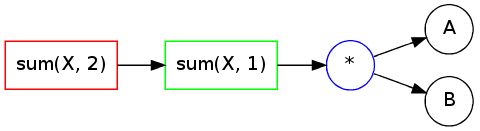
\includegraphics[width=0.48\textwidth]{imgs/example1_brute.png}\\
  {\bf Is equivalent to:}\\
  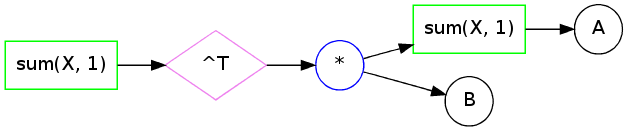
\includegraphics[width=0.48\textwidth]{imgs/example1_opt.png}\\
  \caption{Example of two equivalent mathematical expressions. It states that
  $\sum_{i,j} \sum_k A_{i, k}B_{k, j} = \sum_{j} \sum_k (\sum_i A_{i, k})B_{k, j})$ \cite{zaremba2014learning}.
  This is a toy example, and cited paper contains more sophisticated examples.}
  \label{fig:ident}
\end{figure}


\section{Interface learning}
\label{sec:interface}
Neural networks are a very powerful statistical models, however
some concepts might be very difficult for them to express.
For instance, nesting seems to be a very common operation, that
allows to deal with (1) object hierarchy, (2) natural language parsing,
and (3) compositionality. It would be best to provide stack as an external
interface to the neural network. Neural network should be able to learn how
to use such interface. 

External interfaces could enhance neural networks capabilities, and also provide
access to external resources, and datasets.
There are few other interfaces that could be very useful:
\begin{itemize}
  \item stack
  \item FIFO
  \item an external memory \cite{weston2014memory, graves2014neural}
  \item search engine
  \item database
  \item execution environment like python interpreter
\end{itemize}


State space of many interfaces is massive (e.g. all possible search queries).
Moreover, external interfaces are not-differentiable, 
This obstacles could potentially be addressed by learning a differentiable 
model that describes them (e.g. neural network). Neural network would simulate such 
external interface for purpose of being differentiable.
Some of work in area of interface learning is under progress. It is one of my major projects now.


\section{Small sample complexity}
Current deep learning systems suffer of large sample complexity. Such 
high sample complexity hinders potential use of the systems in online 
learning setting (e.g. robots). It’s expected that during the initial phase of 
learning any system without prior knowledge would need to consume a large number of samples. 
We hope that over the time of training, sample complexity should drop. However, this is 
not observed in a current systems. I propose several approaches how sample complexity can be decreased. 
Meta-optimizer (Subsection \ref{subsec:meta}) is the target solution. Moreover, I propose some intermediate solutions, that can potentially
decrease sample complexity.

\subsection{Automatic derivation of better models}
Neural networks are designed ad-hoc. People have only some partial intuition
regarding how to build high prediction performance systems. 
One way of addressing this issue would be to
fully understand why, and how models work. However, it is unclear if it is even 
possible (maybe best explanation is a model itself). I would like to automatically
explore large space of models, and evaluate them on various tasks. 
This involves connectivity, activation functions, and hyper-parameters.
I would optimize it with genetic programming.
This work is under progress. It is one of my major projects now.


\subsection{Augmentation marginalization}
For simplicity of explanation, we focus on computer vision tasks.


We often train neural networks for multiple epochs, while the same 
samples are presented multiple times. The best performance is
achieved when samples are slightly modified over the course of training.
In case of computer vision, it is done by jittering images, rotating
them, and so on. This is known as data-augmentation. 
Theoretically, a full image contains information about all updates obtained
with all possible augmented samples. More formally, let $x$ be an image, $y$ its label and
$x_1, x_2 \dots x_k$, are its augmented copies. $L$ is a loss function, and $\theta_i$ are parameters at step $i$.
I would like to
predict with $x$ sum of derivatives for all data augmentations:
\begin{align}
f(x, \theta_1) = \sum_{i=1}^k \partial_\theta L(x_k, y, \theta_i)
\end{align}

Instead of following gradient of $\partial_\theta L(x, y, \theta_1)$, we could
follow $f(x, \theta_1)$.
This could improve learning speed, as a single sample would provide
information about it's all augmented copies. 


Function $f$ might have its own parameters, and I would like to model it 
as a neural network. We could train it in supervised fashion. The main issue
is how to avoid explosion of parameters in $f$. 


\subsection{One-shot learning objective}
Human is able to recognize a new object by seeing them just once.
Contemporary deep learning systems are far from it. They need hundreds or
even thousands of instances to make use out of it. 
We propose a new formulation of neural network training that focus on training
toward the one-shot learning objective. 


We achieve it by training neural network to predict parameters of a neural network. 
More formally, let $\phi(x, W_{in}, \theta) = (y, W_{y})$ be a neural network parametrized
by $\theta$. Weights $W_{in} \in \mathbb{R}^{f \times l}$ are a top layer weights, where
$f$ is a top layer feature size, and $l$ is a number of labels. $W_{y} \in \mathbb{R}^f$ is a
single weight vector used to predict class $y$.



For a given new class $x', y'$, we compute $_, W_{y'} = \phi(x', None, \theta)$ to produce weights $W_{y'}$. 
We use this weights to classify
other objects belonging to the class $y'$.



This work is under progress. It is supervised by my collaborators Elias Bingham, and Brenden Lake.

\subsection{Meta-optimizer}
\label{subsec:meta}
I would like to build a meta-optimizer that would be used to train neural network.
Such optimizer would consume gradients of a neural network, 
and would decide on the next update step. Optimizer itself could be parameterized 
with a neural network. Proper weights of meta-optimizer should be able to simulate any first order, gradient-based, 
learning algorithm like SGD, momentum, LBFGs etc. This implies that meta-optimizer should 
subsume all first order, gradient-based optimization techniques. Trained meta-optimizer 
could update the network in a much more clever way, and a single sample could provide enough knowledge.
This work is under progress. It is supervised by my collaborator Rahul Krishnan, and Anna Choromanska.

\section{Discussion}
Tackling aforementioned problems would take us much closer to the
real intelligent systems, and defines for me the three main pillars 
of artificial intelligence. However, there are many other problems, which 
would need to be solved and integrate to achieve fully 
intelligent system, e.g. navigation, learning by imitation, cooperation, and many others.
However, I think that, all that skills can be integrated by means of external interface, and
don't have to be modeled in any special way. For instance, navigation skill could emerge 
as an use two interfaces (1) GPS location interface, and (2) an external memory.


\section{Disclaimer}
This is my personal opinion, and it shouldn't be judged in a scientific way.


I strongly believe that creation of artificial intelligence is potentially
dangerous. However, I think, that more dangerous is avoiding to create it.
We exhaust resources of our planet in rapid fashion, and lack of resources 
leads to wars. The only way to prevent it is to have abundance of resources.
Artificial intelligence could provide abundance of all resources.


\bibliography{bibliography}
\bibliographystyle{icml2014}

\end{document} 

